\documentclass[11pt,a4paper]{article}

\usepackage[margin=1in]{geometry}
\usepackage{mathptmx}
\usepackage{amsmath}
\usepackage{amssymb}
\usepackage{amsthm}
\usepackage{braket}
\usepackage{tikz}
\usepackage{quantikz}
\usepackage{enumitem}
\usepackage{hyperref}
\usepackage{xcolor}

\definecolor{circuitblue}{RGB}{40,80,160}

\hypersetup{
    colorlinks=true,
    linkcolor=circuitblue,
    urlcolor=circuitblue,
    citecolor=circuitblue
}

\theoremstyle{definition}
\newtheorem{definition}{Definition}[section]
\newtheorem{example}{Example}[section]
\newtheorem{theorem}{Theorem}[section]

\theoremstyle{remark}
\newtheorem*{intuition}{Intuition}
\newtheorem*{keypoint}{Key Point}

\pagestyle{plain}

\setlength{\parindent}{0pt}
\setlength{\parskip}{6pt}

\begin{document}

\begin{center}
    {\LARGE \textbf{Introduction and Applications of Quantum Models}}\\[8pt]
    {\large QML}\\[12pt]
    \hrule
\end{center}

\vspace{12pt}
\tableofcontents
\newpage

%% ========================================================
\section{Overview}
%% ========================================================

weve spent the last several lectures building up the theory --- variational circuits, feature maps, kernels, expressibility. now its time to zoom out and ask: wt can u actually \emph{do} with all this? wt kinds of problems can quantum models solve, and which approaches r best for which tasks?

this lecture is a survey-style overview. well taxonomize quantum ML models, walk through how they apply to classification, regression, generative modeling, and reinforcement learning, then look at some of the most interesting architectural ideas (data reuploading, transfer learning, hybrid systems). well finish with a blunt assessment of where real-world QML applications actually stand.

tbh this is the lecture where we connect theory to practice. some of it is exciting, some of it is sobering. thats the state of the field right now.

%% ========================================================
\section{Taxonomy of QML Models}
%% ========================================================

before diving into specific applications, lets organize the landscape. there r broadly three paradigms for quantum ML:

\subsection{The Three Paradigms}

\begin{definition}[Quantum Kernel Methods]
quantum kernel methods use a quantum computer only to evaluate a kernel function $k(x_i, x_j) = |\braket{\phi(x_i)|\phi(x_j)}|^2$, then feed the kernel matrix to a classical ML algorithm (SVM, kernel ridge regression, etc.). no variational optimization on the quantum device.
\end{definition}

\begin{definition}[Variational (Hybrid) Methods]
variational methods use a parameterized quantum circuit $U(\theta, x)$ as the model, with parameters $\theta$ optimized via a classical-quantum feedback loop. the quantum device evaluates the model, the classical computer updates parameters.
\end{definition}

\begin{definition}[Fault-Tolerant Quantum ML]
fault-tolerant algorithms assume access to error-corrected qubits and can run deep circuits. examples include quantum PCA (lloyd et al. 2014), quantum sampling (kerenidis-prakash), HHL-based methods. these need thousands to millions of logical qubits.
\end{definition}

\begin{intuition}
think of it like a spectrum of quantum resource requirements. kernel methods need the least (just state prep + measurement), variational methods need moderate resources (parameterized circuits + optimization), and fault-tolerant methods need the most (deep circuits, error correction). we r currently in the ``variational era'' bcs thats wt NISQ hardware can handle.
\end{intuition}

\subsection{Comparison Table}

\begin{center}
\renewcommand{\arraystretch}{1.4}
\begin{tabular}{|p{3cm}|p{3.5cm}|p{3.5cm}|p{3.5cm}|}
\hline
\textbf{Property} & \textbf{Kernel Methods} & \textbf{Variational} & \textbf{Fault-Tolerant} \\
\hline
hardware era & NISQ & NISQ & post-NISQ \\
\hline
circuit depth & shallow (fixed) & moderate (optimized) & deep (algorithmic) \\
\hline
classical optimization & SVM/KRR (convex) & gradient descent (non-convex) & minimal \\
\hline
trainability & guaranteed (convex) & barren plateaus risk & N/A (algorithmic) \\
\hline
expressiveness & fixed by kernel & tunable via ansatz & full quantum \\
\hline
data encoding & feature map circuit & embedded in ansatz & amplitude encoding \\
\hline
scaling bottleneck & kernel matrix $O(n^2)$ & gradient estimation & qubit count + error correction \\
\hline
provable advantage & yes (liu et al. 2021) & limited results & yes (for specific tasks) \\
\hline
\end{tabular}
\end{center}

\begin{keypoint}
no single paradigm dominates. kernel methods have the best theoretical guarantees but scale poorly with dataset size. variational methods r most flexible but face trainability issues (more on this in lecture 16). fault-tolerant methods have the strongest advantages but need hardware we dont have yet.
\end{keypoint}

%% ========================================================
\section{Quantum Models for Classification}
%% ========================================================

classification is the most studied task in QML, and for good reason --- its clean, well-defined, and easy to benchmark.

\subsection{Variational Quantum Classifier (VQC)}

the VQC is the workhorse of near-term quantum classification. recall the structure:

\begin{enumerate}[label=(\roman*)]
    \item encode classical data $x$ into quantum state via feature map $S(x)$
    \item apply parameterized unitary $W(\theta)$
    \item measure expectation value $\langle Z \rangle$ or similar observable
    \item threshold to get class label
\end{enumerate}

the prediction function is:
\begin{equation}
    f(x; \theta) = \bra{0} S^\dagger(x) W^\dagger(\theta) \, M \, W(\theta) S(x) \ket{0}
\end{equation}
where $M$ is a measurement observable (often $Z_0$ for binary classification).

training objective --- minimize cross-entropy or hinge loss:
\begin{equation}
    \mathcal{L}(\theta) = \frac{1}{N} \sum_{i=1}^{N} \ell\big(y_i, f(x_i; \theta)\big)
\end{equation}

\begin{example}
for binary classification with labels $y \in \{-1, +1\}$ and hinge loss:
\[
\ell(y, \hat{y}) = \max(0, 1 - y \cdot \hat{y})
\]
this is exactly a quantum version of a soft-margin SVM in the variational picture.
\end{example}

\subsection{Quantum Support Vector Classifier (QSVC)}

the kernel approach to classification. u compute the quantum kernel matrix:
\begin{equation}
    K_{ij} = |\bra{0} S^\dagger(x_i) S(x_j) \ket{0}|^2
\end{equation}
then solve the standard SVM dual problem:
\begin{equation}
    \max_{\alpha} \sum_i \alpha_i - \frac{1}{2} \sum_{i,j} \alpha_i \alpha_j y_i y_j K_{ij}
\end{equation}
subject to $0 \leq \alpha_i \leq C$ and $\sum_i \alpha_i y_i = 0$.

\begin{keypoint}
the advantage of QSVC over VQC: the optimization is \emph{convex}. no barren plateaus, no local minima. the disadvantage: u need to compute the full $n \times n$ kernel matrix, which takes $O(n^2)$ quantum circuit evaluations. for large datasets this is a killer.
\end{keypoint}

\subsection{Comparison of Classification Approaches}

\begin{center}
\renewcommand{\arraystretch}{1.3}
\begin{tabular}{|l|c|c|c|}
\hline
\textbf{Method} & \textbf{Training} & \textbf{Prediction} & \textbf{Best For} \\
\hline
VQC & non-convex opt & 1 circuit eval & medium datasets \\
\hline
QSVC & convex (SVM) & $O(n_{sv})$ evals & small datasets \\
\hline
QNN (deep) & non-convex opt & 1 circuit eval & complex patterns \\
\hline
projected kernel & convex + classical & classical & large datasets \\
\hline
\end{tabular}
\end{center}

the projected kernel method (huang et al. 2021) is worth noting: instead of using the fidelity kernel $|\braket{\phi(x)|\phi(y)}|^2$, u measure individual qubit expectation values and use those as classical features. this avoids the $O(n^2)$ kernel matrix computation and can be combined with any classical ML method.

\begin{equation}
    \text{projected features: } \tilde{\phi}(x) = \big(\langle Z_1 \rangle_x, \langle Z_2 \rangle_x, \ldots, \langle Z_n \rangle_x, \langle Z_1 Z_2 \rangle_x, \ldots\big)
\end{equation}

%% ========================================================
\section{Quantum Models for Regression}
%% ========================================================

regression is less studied than classification in QML but follows similar principles.

\subsection{Variational Quantum Regressor (VQR)}

same circuit structure as VQC, but now the output is continuous:
\begin{equation}
    f(x; \theta) = \bra{0} S^\dagger(x) W^\dagger(\theta) \, M \, W(\theta) S(x) \ket{0} \in [-1, 1]
\end{equation}

u can rescale to arbitrary range: $\hat{y} = a \cdot f(x; \theta) + b$ where $a, b$ r learnable or fixed.

training uses MSE loss:
\begin{equation}
    \mathcal{L}(\theta) = \frac{1}{N} \sum_{i=1}^{N} \big(y_i - f(x_i; \theta)\big)^2
\end{equation}

\begin{intuition}
theres smtg subtle here. bcs the output of a quantum measurement is bounded $[-1, 1]$ (for expectation of pauli observables), VQR naturally produces bounded predictions. this can be a feature (built-in regularization) or a bug (cant predict extreme values) depending on ur task.
\end{intuition}

\subsection{Quantum Kernel Ridge Regression (QKRR)}

the kernel approach to regression. given quantum kernel matrix $K$, solve:
\begin{equation}
    \hat{\alpha} = (K + \lambda I)^{-1} y
\end{equation}
where $\lambda > 0$ is the regularization parameter. prediction for new point:
\begin{equation}
    \hat{y}(x_*) = \sum_{i=1}^{N} \hat{\alpha}_i \, k(x_i, x_*)
\end{equation}

this is identical to classical kernel ridge regression but with a quantum kernel. the solution is unique (no local minima), and the regularization $\lambda$ prevents overfitting.

\begin{theorem}[Representer Theorem for QKRR]
the optimal predictor in the RKHS associated with quantum kernel $k$ lies in the span of the training kernel evaluations:
\[
f^*(x) = \sum_{i=1}^{N} \alpha_i^* \, k(x_i, x)
\]
this holds regardless of the loss function (as long as its monotonically increasing in $\|f\|_{\mathcal{H}}$).
\end{theorem}

\begin{example}
QKRR for fitting a 1D function. encode $x \in [0, 2\pi]$ with:
\[
S(x) = \prod_{j=1}^{n} R_Z(x) R_Y(x^2) \cdot \text{CNOT layer}
\]
the quantum kernel captures nonlinear correlations that would require high-degree polynomials classically. for smooth functions with periodic structure, quantum kernels can be remarkably efficient.
\end{example}

\subsection{Multi-Output Regression}

for vector-valued regression $y \in \mathbb{R}^m$, u have two options:

\begin{enumerate}[label=\arabic*.]
    \item \textbf{multiple observables}: measure different pauli operators for each output dimension
    \begin{equation}
        f_k(x; \theta) = \bra{\psi(x, \theta)} M_k \ket{\psi(x, \theta)}, \quad k = 1, \ldots, m
    \end{equation}

    \item \textbf{multiple circuits}: use a separate parameterized circuit for each output (more parameters, more flexible, more expensive)
\end{enumerate}

the first approach is more parameter-efficient but couples all outputs through shared circuit parameters. the second is more flexible but scales linearly in the number of outputs.

%% ========================================================
\section{Quantum Models for Generative Tasks}
%% ========================================================

generative modeling is arguably the most ``quantum-native'' ML task, bcs quantum mechanics is fundamentally about probability distributions.

\subsection{Born Machines}

\begin{definition}[Born Machine]
a Born machine is a generative model that directly uses the Born rule to define a probability distribution:
\begin{equation}
    p_\theta(x) = |\bra{x} U(\theta) \ket{0^n}|^2
\end{equation}
where $U(\theta)$ is a parameterized quantum circuit and $\ket{x}$ is a computational basis state.
\end{definition}

this is beautiful in its simplicity: the quantum circuit directly \emph{is} the generative model. sampling is trivial --- just run the circuit and measure. the hard part is training.

training approaches:
\begin{enumerate}[label=(\roman*)]
    \item \textbf{MLE}: maximize $\sum_i \log p_\theta(x_i)$ --- but computing $p_\theta(x)$ requires exponentially many measurements for general circuits
    \item \textbf{MMD minimization}: minimize maximum mean discrepancy between model and data distributions
    \begin{equation}
        \text{MMD}^2 = \mathbb{E}_{x,x' \sim p_{\text{data}}}[k(x,x')] - 2\mathbb{E}_{x \sim p_{\text{data}}, y \sim p_\theta}[k(x,y)] + \mathbb{E}_{y,y' \sim p_\theta}[k(y,y')]
    \end{equation}
    \item \textbf{Stein discrepancy}: uses score function, avoids computing normalization
\end{enumerate}

\begin{intuition}
born machines can represent distributions that r exponentially hard for classical models. the amplitude of an $n$-qubit state has $2^n$ components, so a Born machine over $n$ bits has a ``model capacity'' thats exponential in $n$. whether this helps for real-world distributions is an open question.
\end{intuition}

\subsection{Quantum GANs (qGANs)}

quantum GANs follow the classical GAN framework but replace one or both networks with quantum circuits:

\begin{enumerate}[label=\arabic*.]
    \item \textbf{quantum generator, classical discriminator}: generator is $U(\theta_G)\ket{0}$, measured samples fed to classical discriminator
    \item \textbf{quantum generator, quantum discriminator}: both r quantum circuits, discriminator tries to distinguish real data (loaded into quantum state) from generated samples
    \item \textbf{classical generator, quantum discriminator}: less common, but the quantum discriminator might detect patterns the classical one misses
\end{enumerate}

the minimax game:
\begin{equation}
    \min_{\theta_G} \max_{\theta_D} \; \mathbb{E}_{x \sim p_{\text{data}}}[\log D_{\theta_D}(x)] + \mathbb{E}_{z \sim p_z}[\log(1 - D_{\theta_D}(G_{\theta_G}(z)))]
\end{equation}

for the fully quantum version, the discriminator is a quantum circuit that outputs a single qubit measurement:
\begin{equation}
    D_{\theta_D}(\rho) = \text{Tr}\big[M \, V(\theta_D) \rho \, V^\dagger(\theta_D)\big]
\end{equation}

\begin{keypoint}
qGANs have been demonstrated for loading probability distributions into quantum states (zoufal et al. 2019). the practical use case isnt generating cat pictures --- its efficiently preparing quantum states that represent classical probability distributions, which is useful as a subroutine in other quantum algorithms.
\end{keypoint}

%% ========================================================
\section{Quantum Models for Reinforcement Learning}
%% ========================================================

quantum reinforcement learning (QRL) is the least mature subfield of QML, but has some interesting ideas.

\subsection{The Setup}

in RL, an agent interacts with an environment through a policy $\pi(a|s)$ that maps states to action probabilities. the goal is to maximize expected cumulative reward:
\begin{equation}
    J(\theta) = \mathbb{E}_{\tau \sim \pi_\theta}\left[\sum_{t=0}^{T} \gamma^t r_t\right]
\end{equation}

a quantum policy uses a PQC to parameterize $\pi$:
\begin{equation}
    \pi_\theta(a|s) = |\bra{a} U(\theta, s) \ket{0}|^2
\end{equation}
where the state $s$ is encoded into the circuit and different measurement outcomes correspond to different actions.

\subsection{Quantum Policy Gradient}

the REINFORCE algorithm adapts directly:
\begin{equation}
    \nabla_\theta J = \mathbb{E}_{\tau \sim \pi_\theta}\left[\sum_{t=0}^{T} \nabla_\theta \log \pi_\theta(a_t | s_t) \cdot G_t\right]
\end{equation}
where $G_t = \sum_{k=t}^{T} \gamma^{k-t} r_k$ is the return.

bcs we can use the parameter shift rule to compute $\nabla_\theta \log \pi_\theta$, the quantum policy gradient is well-defined. the circuit acts as a function approximator for the policy, similar to how neural networks r used in classical deep RL.

\begin{example}
quantum policy for CartPole (skolik et al. 2022): 4 state variables (cart position, velocity, pole angle, angular velocity) encoded into a 4-qubit circuit. measurement of first qubit determines action (left/right). with just $\sim$20 parameters, the quantum agent matches the performance of a classical neural network with $\sim$100 parameters.
\end{example}

\begin{intuition}
the potential advantage of quantum RL is parameter efficiency: quantum circuits can represent complex policies with fewer parameters than classical networks. whether this translates to faster learning or better generalization is still debated. the main challenge is that RL already has high variance in gradient estimates, and quantum measurement noise makes it worse.
\end{intuition}

%% ========================================================
\section{Data Reuploading}
%% ========================================================

this is one of the most important architectural ideas in QML. introduced by p\'erez-salinas et al. (2020), data reuploading turns a single-qubit circuit into a universal classifier.

\subsection{The Core Idea}

instead of encoding data once at the beginning, encode it \emph{multiple times} throughout the circuit, interleaved with trainable gates:

\begin{equation}
    U(\theta, x) = \prod_{l=1}^{L} \Big[ W_l(\theta_l) \cdot S(x) \Big]
\end{equation}

each ``layer'' re-encodes the data and applies a trainable rotation. the key insight: this is analogous to a classical neural network where each layer applies a nonlinear activation to a linear transformation of the input.

\subsection{Data Reuploading Circuit}

\begin{center}
\begin{quantikz}
\lstick{$\ket{0}$} & \gate{R(\vec{x})} & \gate{R(\vec{\theta}_1)} & \gate{R(\vec{x})} & \gate{R(\vec{\theta}_2)} & \gate{R(\vec{x})} & \gate{R(\vec{\theta}_3)} & \meter{}
\end{quantikz}
\end{center}

for the single-qubit case, each gate is a general $SU(2)$ rotation:
\begin{equation}
    R(\vec{v}) = \exp\left(-i \frac{v_1 X + v_2 Y + v_3 Z}{2}\right)
\end{equation}
so the encoding gate uses $\vec{v} = \vec{x}$ and the trainable gate uses $\vec{v} = \vec{\theta}_l$.

for multi-qubit data reuploading, add entangling layers between re-uploads:

\begin{center}
\begin{quantikz}
\lstick{$\ket{0}$} & \gate{R_Y(x_1)} & \gate{R_Y(\theta_1)} & \ctrl{1} & \qw      & \gate{R_Y(x_1)} & \gate{R_Y(\theta_4)} & \ctrl{1} & \qw      & \meter{} \\
\lstick{$\ket{0}$} & \gate{R_Y(x_2)} & \gate{R_Y(\theta_2)} & \targ{}  & \ctrl{1} & \gate{R_Y(x_2)} & \gate{R_Y(\theta_5)} & \targ{}  & \ctrl{1} & \meter{} \\
\lstick{$\ket{0}$} & \gate{R_Y(x_3)} & \gate{R_Y(\theta_3)} & \qw      & \targ{}  & \gate{R_Y(x_3)} & \gate{R_Y(\theta_6)} & \qw      & \targ{}  & \meter{}
\end{quantikz}
\end{center}

\subsection{Why It Works: Fourier Analysis}

the connection to fourier analysis (schuld, sweke, meyer 2021) explains everything. a data reuploading circuit with $L$ layers computes:
\begin{equation}
    f(x; \theta) = \sum_{\omega \in \Omega} c_\omega(\theta) \, e^{i\omega x}
\end{equation}
where $\Omega$ is the set of accessible frequencies determined by the encoding gates.

\begin{theorem}[Universal Approximation via Data Reuploading]
a single-qubit data reuploading circuit with $L$ layers can represent any trigonometric polynomial of degree up to $L$:
\[
f(x) = \sum_{k=-L}^{L} c_k \, e^{ikx}
\]
by choosing appropriate trainable parameters $\theta_1, \ldots, \theta_L$. as $L \to \infty$, this becomes dense in continuous functions on $[0, 2\pi]$ (by standard fourier analysis).
\end{theorem}

\begin{intuition}
each data re-upload adds one more frequency to the fourier spectrum. so $L$ layers of reuploading give u access to frequencies $\{-L, -L+1, \ldots, L\}$. the trainable parameters control the fourier coefficients $c_k$. more layers = higher frequency components = ability to fit more complex functions. this is directly analogous to increasing the width/depth of a classical neural network.
\end{intuition}

\begin{keypoint}
data reuploading solved a fundamental limitation of single-encoding circuits. with data encoded only once, a PQC computes a restricted class of functions (limited frequencies). with reuploading, the function class grows with circuit depth, eventually becoming universal. this is wt makes quantum models practical function approximators.
\end{keypoint}

\subsection{Practical Considerations}

\begin{itemize}
    \item \textbf{number of layers $L$}: more layers = more expressive but harder to train (deeper circuit, more parameters, potential barren plateaus)
    \item \textbf{encoding gate choice}: $R_Z(x)$ gives frequencies $\{-1, 0, 1\}$ per qubit per layer. using $R_Z(x) R_Y(x)$ can give richer frequency spectra
    \item \textbf{multi-qubit scaling}: with $n$ qubits and $L$ layers, the frequency spectrum grows combinatorially. this is where quantum advantage might come from
    \item \textbf{entanglement between re-uploads}: CNOT layers between data re-uploads create correlations between qubits, enabling the circuit to capture multi-variate interactions
\end{itemize}

%% ========================================================
\section{Quantum Transfer Learning}
%% ========================================================

transfer learning is one of the most successful ideas in classical ML: take a model pre-trained on a large dataset, replace the last layer, and fine-tune on ur specific task. the quantum version adapts this by replacing the last layer with a quantum circuit.

\subsection{The Architecture}

mari et al. (2020) proposed the following pipeline:

\begin{enumerate}[label=\arabic*.]
    \item take a pre-trained classical CNN (e.g., ResNet-18 trained on ImageNet)
    \item remove the final classification layer
    \item add a dimensionality reduction layer (from $d$ features to $n$ features, where $n$ = number of qubits)
    \item feed the reduced features into a variational quantum circuit
    \item measure to get class predictions
\end{enumerate}

\begin{equation}
    \hat{y} = \text{Measure}\Big[ U(\theta) \cdot S\big(\text{Reduce}(\text{CNN}(x))\big) \ket{0^n} \Big]
\end{equation}

\subsection{Architecture Diagram}

\begin{center}
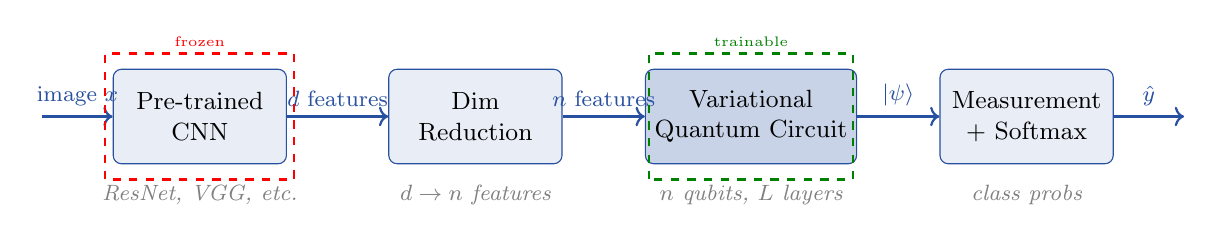
\begin{tikzpicture}[
    block/.style={rectangle, draw=circuitblue, fill=circuitblue!10,
        minimum width=2.2cm, minimum height=1.2cm, rounded corners=3pt,
        font=\small, text centered, align=center},
    arrow/.style={->, thick, circuitblue},
    label/.style={font=\footnotesize\itshape, text=gray}
]

% Classical CNN
\node[block] (cnn) at (0,0) {Pre-trained\\CNN};
\node[label] at (0, -1.0) {ResNet, VGG, etc.};

% Dim reduction
\node[block] (reduce) at (3.5,0) {Dim\\Reduction};
\node[label] at (3.5, -1.0) {$d \to n$ features};

% Quantum circuit
\node[block, fill=circuitblue!25] (qc) at (7,0) {Variational\\Quantum Circuit};
\node[label] at (7, -1.0) {$n$ qubits, $L$ layers};

% Measurement
\node[block] (meas) at (10.5,0) {Measurement\\+ Softmax};
\node[label] at (10.5, -1.0) {class probs};

% Arrows
\draw[arrow] (-2, 0) -- (cnn) node[midway, above, font=\footnotesize] {image $x$};
\draw[arrow] (cnn) -- (reduce) node[midway, above, font=\footnotesize] {$d$ features};
\draw[arrow] (reduce) -- (qc) node[midway, above, font=\footnotesize] {$n$ features};
\draw[arrow] (qc) -- (meas) node[midway, above, font=\footnotesize] {$\ket{\psi}$};
\draw[arrow] (meas) -- (12.5, 0) node[midway, above, font=\footnotesize] {$\hat{y}$};

% Freeze/train indicators
\draw[thick, red, dashed] (-1.2, -0.8) rectangle (1.2, 0.8);
\node[font=\tiny, red] at (0, 0.95) {frozen};

\draw[thick, green!50!black, dashed] (5.7, -0.8) rectangle (8.3, 0.8);
\node[font=\tiny, green!50!black] at (7, 0.95) {trainable};

\end{tikzpicture}
\end{center}

\subsection{Why This Makes Sense}

\begin{itemize}
    \item \textbf{classical CNNs r great feature extractors}: billions of parameters trained on millions of images have learned incredibly useful representations. no quantum model comes close (yet)
    \item \textbf{quantum circuits add expressive power at the decision boundary}: even a small quantum circuit (4-8 qubits) can implement complex decision functions in the feature space
    \item \textbf{few parameters to train}: the quantum circuit might have 20-50 parameters, so u need very little data to fine-tune
    \item \textbf{practical on current hardware}: only need a few qubits, shallow circuits
\end{itemize}

\begin{example}
transfer learning for medical image classification (mari et al. 2020): ResNet-18 pre-trained on ImageNet, features reduced from 512 to 4, fed into 4-qubit variational circuit. on a binary classification task (ants vs. bees), the hybrid model achieved 96\% accuracy, matching the fully classical fine-tuned model. the quantum circuit had only 24 trainable parameters.
\end{example}

\begin{keypoint}
quantum transfer learning is arguably the most practical QML architecture for real-world image classification right now. it leverages the best of classical ML (feature extraction) and only uses the quantum circuit where it matters (decision making). the downside: its hard to claim quantum advantage when 99\% of the work is done classically.
\end{keypoint}

%% ========================================================
\section{Hybrid Classical-Quantum Architectures}
%% ========================================================

there r many ways to combine classical and quantum computation beyond transfer learning. lets categorize them.

\subsection{Architecture Patterns}

\begin{definition}[Quantum-Classical Hybrid Architectures]
we identify four main patterns:
\begin{enumerate}[label=(\alph*)]
    \item \textbf{quantum layer in classical network}: embed a quantum circuit as one layer in a classical deep network. classical layers before and after. this is the ``dressed quantum circuit'' approach
    \item \textbf{classical pre/post-processing}: classical networks handle data preprocessing and output post-processing, quantum circuit does the core computation
    \item \textbf{parallel quantum-classical}: run classical and quantum models on the same input, combine their outputs (ensemble-like)
    \item \textbf{alternating quantum-classical}: alternate between quantum and classical processing layers, passing data back and forth
\end{enumerate}
\end{definition}

\subsection{The Dressed Quantum Circuit}

the most general hybrid architecture (mari et al. 2020):
\begin{equation}
    f(x) = g_{\text{post}}\Big( \text{Measure}\big[ U(\theta) \, S(g_{\text{pre}}(x)) \ket{0^n} \big] \Big)
\end{equation}
where $g_{\text{pre}}$ and $g_{\text{post}}$ r classical neural networks.

this gives u the best of both worlds:
\begin{itemize}
    \item $g_{\text{pre}}$: dimensionality reduction, feature extraction, normalization
    \item $U(\theta)$: quantum processing in hilbert space
    \item $g_{\text{post}}$: mapping quantum outputs to desired format (softmax for classification, rescaling for regression, etc.)
\end{itemize}

the entire pipeline is end-to-end differentiable (using parameter shift rule for the quantum part), so u can train everything jointly with backpropagation.

\subsection{Practical Hybrid Training}

\begin{enumerate}[label=\arabic*.]
    \item \textbf{joint training}: train all parameters (classical + quantum) simultaneously. requires careful learning rate tuning --- quantum parameters often need different learning rates than classical ones
    \item \textbf{alternating training}: freeze classical, train quantum, then freeze quantum, train classical. simpler but slower convergence
    \item \textbf{pre-train then fine-tune}: pre-train classical parts, then fine-tune quantum circuit. this is the transfer learning approach
\end{enumerate}

\begin{keypoint}
in practice, the best results come from joint training with separate learning rates: $\eta_{\text{classical}} \sim 10^{-3}$ (Adam) and $\eta_{\text{quantum}} \sim 10^{-1}$ to $10^{-2}$ (often plain SGD works fine for the quantum part). quantum parameters tend to have smoother loss landscapes and benefit from larger step sizes.
\end{keypoint}

%% ========================================================
\section{Real-World Application Areas}
%% ========================================================

lets survey where QML is being applied (or at least attempted).

\subsection{Finance}

finance is one of the most active areas for QML research, driven by the potential economic value and the mathematical sophistication of financial models.

\textbf{portfolio optimization}: given $n$ assets with expected returns $\mu$ and covariance matrix $\Sigma$, the markowitz problem is:
\begin{equation}
    \min_w \; w^T \Sigma w - \lambda \mu^T w \quad \text{s.t.} \quad \sum_i w_i = 1, \; w_i \geq 0
\end{equation}

quantum approaches:
\begin{itemize}
    \item QAOA for discrete portfolio optimization (selecting $k$ from $n$ assets)
    \item VQE-based continuous optimization
    \item quantum annealing (D-Wave) for combinatorial variants
\end{itemize}

\textbf{option pricing}: pricing european/asian options requires computing expectations under risk-neutral measure:
\begin{equation}
    V = e^{-rT} \mathbb{E}^Q\big[\text{payoff}(S_T)\big]
\end{equation}

quantum amplitude estimation can achieve quadratic speedup over classical monte carlo: $O(1/\epsilon)$ vs $O(1/\epsilon^2)$. this is one of the most concrete near-term quantum advantages, though the constant factors r still challenging.

\textbf{fraud detection}: QML classifiers (VQC, QSVC) applied to transaction data. results so far: competitive with classical methods on small datasets but no clear advantage. the bottleneck is data encoding.

\subsection{Chemistry and Drug Discovery}

\textbf{molecular simulation}: this is arguably the ``killer app'' for quantum computing, though its more quantum simulation than QML per se. VQE finds ground state energies of molecules:
\begin{equation}
    E_0 = \min_\theta \bra{\psi(\theta)} H \ket{\psi(\theta)}
\end{equation}
where $H$ is the molecular hamiltonian in second quantization.

\textbf{drug discovery pipeline}: quantum models can contribute at several stages:
\begin{itemize}
    \item molecular property prediction (QML classifiers/regressors)
    \item molecular similarity (quantum kernels on molecular fingerprints)
    \item conformer generation (quantum generative models)
    \item binding affinity prediction (hybrid quantum-classical models)
\end{itemize}

\begin{example}
quantum kernel for molecular property prediction (huang et al. 2021): quantum kernels applied to molecular descriptors for predicting solubility. with engineered quantum feature maps that respect molecular symmetries, the quantum kernel matched or slightly exceeded classical kernels (RBF, Tanimoto) on benchmark datasets. the advantage was most pronounced for small training sets ($< 100$ molecules).
\end{example}

\subsection{Optimization}

\textbf{logistics and scheduling}: combinatorial optimization problems (vehicle routing, job-shop scheduling, bin packing) mapped to QUBO formulations and solved with QAOA or quantum annealing.

the QUBO formulation:
\begin{equation}
    \min_z z^T Q z, \quad z \in \{0, 1\}^n
\end{equation}

QAOA maps this to a quantum circuit:
\begin{equation}
    \ket{\psi(\gamma, \beta)} = \prod_{p=1}^{P} e^{-i\beta_p H_M} e^{-i\gamma_p H_C} \ket{+}^{\otimes n}
\end{equation}
where $H_C$ encodes the cost function and $H_M = \sum_i X_i$ is the mixer.

\begin{keypoint}
tbh, for optimization problems, the evidence for quantum advantage is mixed at best. classical solvers (gurobi, CPLEX) r incredibly well-optimized after decades of development. quantum approaches might eventually win for specific problem structures, but we r not there yet.
\end{keypoint}

\subsection{Materials Science}

quantum models for predicting material properties:
\begin{itemize}
    \item band gap prediction using quantum kernels
    \item phase classification of quantum many-body systems
    \item materials discovery via quantum generative models
\end{itemize}

the natural connection: materials r quantum systems, so quantum models might capture relevant physics more naturally than classical ones.

%% ========================================================
\section{Honest Assessment: What Actually Works}
%% ========================================================

time for some real talk. where does QML actually stand?

\subsection{What Works (or at Least Shows Promise)}

\begin{enumerate}[label=\arabic*.]
    \item \textbf{quantum kernels for small datasets}: when u have $< 1000$ data points and the quantum kernel captures relevant structure, QSVC can match or beat classical methods. proven advantage exists for specific synthetic problems (liu et al. 2021)

    \item \textbf{hybrid transfer learning}: practical on current hardware, competitive results on image classification. but the quantum part contributes marginally

    \item \textbf{quantum simulation / VQE}: this is where near-term quantum computers have the clearest path to advantage. not purely ML but uses variational methods

    \item \textbf{generative modeling}: born machines can represent distributions that r provably hard for classical models. practical utility still being demonstrated

    \item \textbf{QAOA for specific problem instances}: some evidence of advantage for certain combinatorial structures, but not general-purpose
\end{enumerate}

\subsection{What Doesnt Work (Yet)}

\begin{enumerate}[label=\arabic*.]
    \item \textbf{QML on big data}: current quantum computers have $\sim$100 noisy qubits. encoding thousands of high-dimensional data points is impractical. classical ML wins by default on big data

    \item \textbf{replacing deep learning}: no quantum model comes close to matching a transformer or modern CNN on standard benchmarks (ImageNet, NLP tasks, etc.). the gap is enormous

    \item \textbf{general-purpose quantum advantage in ML}: no one has demonstrated that a quantum ML model outperforms the best classical model on a practically relevant task with real data

    \item \textbf{quantum RL}: interesting theoretical framework but limited by noisy hardware and high variance. classical RL algorithms r much more mature
\end{enumerate}

\subsection{What Needs More Qubits}

\begin{enumerate}[label=\arabic*.]
    \item \textbf{amplitude encoding of large datasets}: encoding $N$ data points into $\log N$ qubits requires coherent operations that scale polynomially --- currently infeasible for large $N$

    \item \textbf{fault-tolerant QML algorithms}: quantum PCA, quantum sampling, HHL-based methods all need error-corrected qubits. estimated timeline: 5-15 years for useful problem sizes

    \item \textbf{quantum advantage in kernel methods}: the liu et al. result shows advantage exists in principle, but the advantage regime requires circuits that r deeper than current hardware supports with acceptable noise levels
\end{enumerate}

\begin{keypoint}
the honest summary: QML is a field with beautiful theory, some promising near-term applications (especially in quantum chemistry), but no ``smoking gun'' practical advantage yet. the most impactful near-term path is probably hybrid classical-quantum approaches that leverage the strengths of both paradigms. if someone tells u they have quantum advantage on a real ML problem with current hardware, be skeptical and ask to see the comparison with properly tuned classical baselines.
\end{keypoint}

%% ========================================================
\section{Looking Forward}
%% ========================================================

\subsection{Near-Term Opportunities}

\begin{itemize}
    \item \textbf{quantum-inspired classical algorithms}: sometimes the process of designing quantum algorithms inspires better classical ones (e.g., dequantization results by tang 2019). this is valuable even without a quantum computer

    \item \textbf{domain-specific quantum models}: instead of trying to beat classical ML generally, design quantum models that exploit domain-specific structure (e.g., molecular symmetries, lattice geometries)

    \item \textbf{quantum data}: the clearest advantage is for data that comes from quantum systems (quantum sensors, quantum communication, quantum chemistry experiments). here, quantum models have an inherent advantage bcs the data is already quantum

    \item \textbf{better classical simulation}: understanding quantum ML models often leads to better classical simulation techniques, which benefits everyone
\end{itemize}

\subsection{The Path to Practical Advantage}

\begin{equation}
    \text{Practical QML Advantage} = \underbrace{\text{Provable Separation}}_{\text{theory}} + \underbrace{\text{Relevant Problem}}_{\text{application}} + \underbrace{\text{Sufficient Hardware}}_{\text{engineering}}
\end{equation}

we currently have the first ingredient for specific problems, the second is debatable, and the third is years away. but the field is moving fast.

\begin{intuition}
dont be a QML doomer and dont be a QML hype person. the technology is real, the math is beautiful, and specific advantages r provable. the path to practical impact requires patience, honest benchmarking, and a willingness to admit when classical methods r simply better. thats how science works.
\end{intuition}

%% ========================================================
\section{Summary}
%% ========================================================

\begin{enumerate}[label=\arabic*.]
    \item \textbf{taxonomy}: QML splits into kernel methods (convex, limited scale), variational methods (flexible, trainability issues), and fault-tolerant methods (powerful, future hardware)

    \item \textbf{classification}: VQC and QSVC r the workhorses. projected kernels help with scaling. no clear advantage over classical methods on standard benchmarks

    \item \textbf{regression}: VQR and QKRR extend the classification approaches. bounded outputs from quantum measurements r a feature and a limitation

    \item \textbf{generative models}: born machines r quantum-native and can represent hard distributions. qGANs useful for state preparation. training is challenging

    \item \textbf{RL}: quantum policy gradients work in principle but face variance and hardware challenges. parameter efficiency is the main potential win

    \item \textbf{data reuploading}: re-encode data multiple times to increase expressiveness. fourier analysis explains why it works. universal approximation with enough layers

    \item \textbf{transfer learning}: combine classical CNN features with quantum circuits. most practical near-term architecture

    \item \textbf{applications}: finance, chemistry, optimization r the main targets. honest assessment: promising but no smoking gun advantage yet
\end{enumerate}

next lecture we tackle the elephant in the room: barren plateaus and trainability. this is wt determines whether variational QML can actually scale, and its one of the most active research areas in the field.

\end{document}
